\documentclass[../../main.tex]{subfiles}

\begin{document}

\section{Transformers}
\subsection{Introduction}
\autoref{np-fig:cnp-architecture}
The Transformer is a deep learning architecture introduced in \parencite{vaswani2017attention}. It is a sequence-to-sequence model that uses attention to learn the relationships between the input and output sequences.

In this report we will follow the notation that is used in \parencite{vaswani2017attention} where embeddings are represented as rows $\elof{1}{D}$ and all matrix multiplications are right multiplications. Subscripts that are not bolded and lowercase are used to index vectors. Superscripts that are surrounded by parenthesis are used to index the position of a vector/matrix within a sequence, layer or head. 

\subsection{Embedding}

A machine is not capable of understanding wordings, hence we need to transform it into a vector representation called an \emph{embedding}. Let us denote the embedding of the $i$-th word in the input sequence as $\bm{e}\isup{i} \elof{1}{D}$, where $D$ is the feature dimension. The transformer can process these embeddings in \textbf{parallel} so we need a way to encode the position of the word in the sequence. We do this by adding a positional encoding $\bm{p}\isup{i} \elof{1}{D}$ to the embedding $\bm{e}\isup{i}$. The positional encoding is a vector that is unique to the position of the word in the sequence. The positional encoding that is used in \parencite{vaswani2017attention} is given by:

\begin{equation}
	\label{pe}
	\bm{p}_j\isup{i} = \begin{cases}
		\sin\left(\frac{i}{10000^{j/D}}\right) & \text{if } j \text{ is even} \\
		\cos\left(\frac{i}{10000^{(j-1)/D}}\right) & \text{if } j \text{ is odd}
	\end{cases}
\end{equation}

\noi where $j$ is the dimension of the positional encoding. The positional encoding is added to the embedding as follows:

\begin{equation}
	\bm{x}\isup{i} =  \bm{e}\isup{i} + \bm{p}\isup{i} \elof{1}{D}
\end{equation}

\noi These are all stacked together to form the input matrix $\bm{X} \elof{N}{D}$, where $\bm{X}_{i:} = \bm{x}\isup{i}$ and $N$ is the number of words in the input sequence.

\begin{note}[Alternative Positional Encoding]
	There are many ways to go about positional encoding. Another way is to use a learned positional encoding. This is done by adding a learnable vector $\bm{p}\isup{i} \elof{1}{D}$ to the embedding. Alternatively, to achieve translation equivariance, we can use \emph{Relative Positional Encoding} \parencite{shaw2018selfattention, wu2021rethinking}. These positional encoding schemes will be useful when trying to build equivariance into the Transformer model. See 
	\parencite{kazemnejad2019:pencoding} for a comparison of different positional encoding schemes.
\end{note}


\subsection{(Self-)Attention}

The attention mechanism is a way to learn the relationships between the input and output sequences. `Normal' attention infers what the most important word/phrase in an input sentence is which is not very powerful. This is where the idea of \emph{self-attention} comes in. Self-attention is a way to learn the relationships between the words in the input sequence itself (Note when we say attention from now on, we mean self-attention).  The example sentence \texttt{The quick brown fox jumps over the lazy dog} has strong attention between the words like \texttt{fox} and \texttt{jumps} representing an action, \texttt{brown} and \texttt{fox} representing the color of the fox and so on, then there are very weak attentions between words \texttt{quick} and \texttt{dog} representing the lack of relationship between the two words. Using self-attention we can learn these relationships between the words in the input sequence, this gives a powerful mechanism to learn the relationships between the input and output sequences and thus allows the model to learn the translation of the input sequence.

In the transformer models we will used the embeddings $\bm{X} \elof{N}{D}$ as the input to generate a query $\bm{Q} \elof{N}{d_k}$, a key $\bm{K} \elof{N}{d_k}$ and a value $\bm{V} \elof{N}{d_v}$ matrices via a simple linear transformation matrix $\bm{W_q} \elof{D}{d_k}$, $\bm{W_k} \elof{D}{d_k}$ and $\bm{W_v} \elof{D}{d_v}$ respectively. 

\begin{align*}
	\bm{Q} &= \bm{X}\bm{W_q} \elof{N}{d_k}\\
	\bm{K} &= \bm{X}\bm{W_k} \elof{N}{d_k}\\
	\bm{V} &= \bm{X}\bm{W_v} \elof{N}{d_v}
\end{align*}


Where each row of the matrices is the query, key and value vectors for each word in the input sequence. The query represents the word that we want to compare to the other words in the input sequence, to do this we compare it to the key vectors. The value vectors represent the word that we want to output.

The query, key and value matrices are then used to compute the attention matrix $\bm{A} \elof{N}{N}$ as follows:

\begin{equation}
    \bm{A} = \text{softmax}\left(\frac{\bm{Q}\bm{K}^T}{\sqrt{d_k}}\right)
\end{equation}

\noi The intuition behind this is that we want to compute the similarity between the query and the key vectors as such we use the dot product between the query and key vectors. The softmax is used to normalize the attention matrix so that the rows sum to 1. The softmax is also scaled by $\sqrt{d_k}$ to prevent the softmax from saturating. The attention matrix is then used to compute the output matrix $\bm{H} \elof{N}{d_v}$ as follows:

\begin{equation}
    \bm{H} = \bm{A}\bm{V}
\end{equation}

\begin{note}[Attention Mechanisms]

There are many ways to compute the attention matrix $\bm{A}$. The one that is used in the original transformer paper is called \emph{Scaled Dot-Product Attention}. Other attention mechanisms may be of interest, see \parencite{weng2018attention} for a comparison of different attention mechanisms.

\end{note}

The overall attention function for a layer is given by:

\begin{equation}
    \bm{H} =\text{Attention}(\bm{Q}, \bm{K}, \bm{V}) = \text{softmax}\left(\frac{\bm{Q}\bm{K}^T}{\sqrt{d_k}}\right)\bm{V}
\end{equation}

\subsection{Multi-Head Self-Attention}

So far we have only computed the attention matrix $\bm{A}$ once so the model only learns one attention relationship, however, we can take advantage of using multiple attention `heads' in parallel to learn many different attention relationships, this scheme is called the \emph{Multi-Head Attention} (MHSA). 

Each attention head is computed using simple dot product attention of a transformed query, key and value matrix. They are transformed by a simple linear layer (a matrix) which is unique for each head of the MHSA, $\bm{W_q}\isup{i} \elof{d_k}{d_k}$, $\bm{W_k}\isup{i} \elof{d_k}{d_k}$ and $\bm{W_v}\isup{i} \elof{d_v}{d_v}$ where $i \in [1, h]$ for a head count of $h$. Then the attention for the particular head is computed as follows:

\begin{equation}
	\bm{H}\isup{i} = \text{Attention}(\bm{Q}\bm{W_q}\isup{i}, \bm{K}\bm{W_k}\isup{i}, \bm{V}\bm{W_v}\isup{i}) \elof {N}{d_v}
\end{equation}

Then the output of the MHSA is the concatenation of the outputs of each head $\bm{H}\isup{i}$ (stacked on to of each other) multiplied by a learnable matrix $\bm{W_O} \elof{hd_v}{D}$ which transforms the concatenated output to the original dimensionality of the input sequence.

\begin{align*}
	 \text{MHSA}(\bm{Q}, \bm{K}, \bm{V}) &= \text{concat}(\bm{H}\isup{1}; \bm{H}\isup{2}; \dots; \bm{H}\isup{h})\bm{W_O} 
	= \begin{bmatrix}
		\bm{H}\isup{1} \\
		\bm{H}\isup{2} \\
		\vdots \\
		\bm{H}\isup{h}
	\end{bmatrix} \bm{W_O} \elof{N}{D}
\end{align*}

The figure below summarizes the MHSA operation.

\begin{figure}[H]
	\centering
	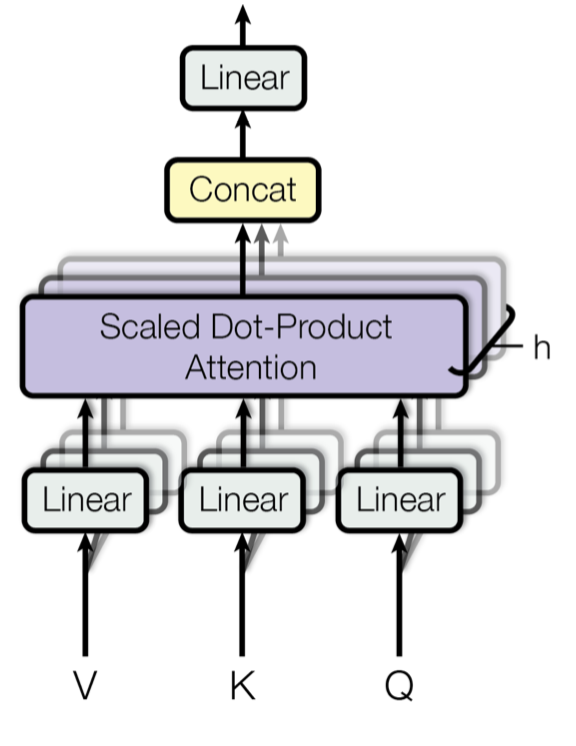
\includegraphics[height=0.4\textwidth]{./mhsa.png}
	\caption{Multi-Head Self-Attention \parencite{vaswani2017attention}}
\end{figure}

\subsection{Encoder}

Now that we have covered the MHSA block, we can move on to the encoder of the transformer.

\begin{figure}[H]
	\centering
	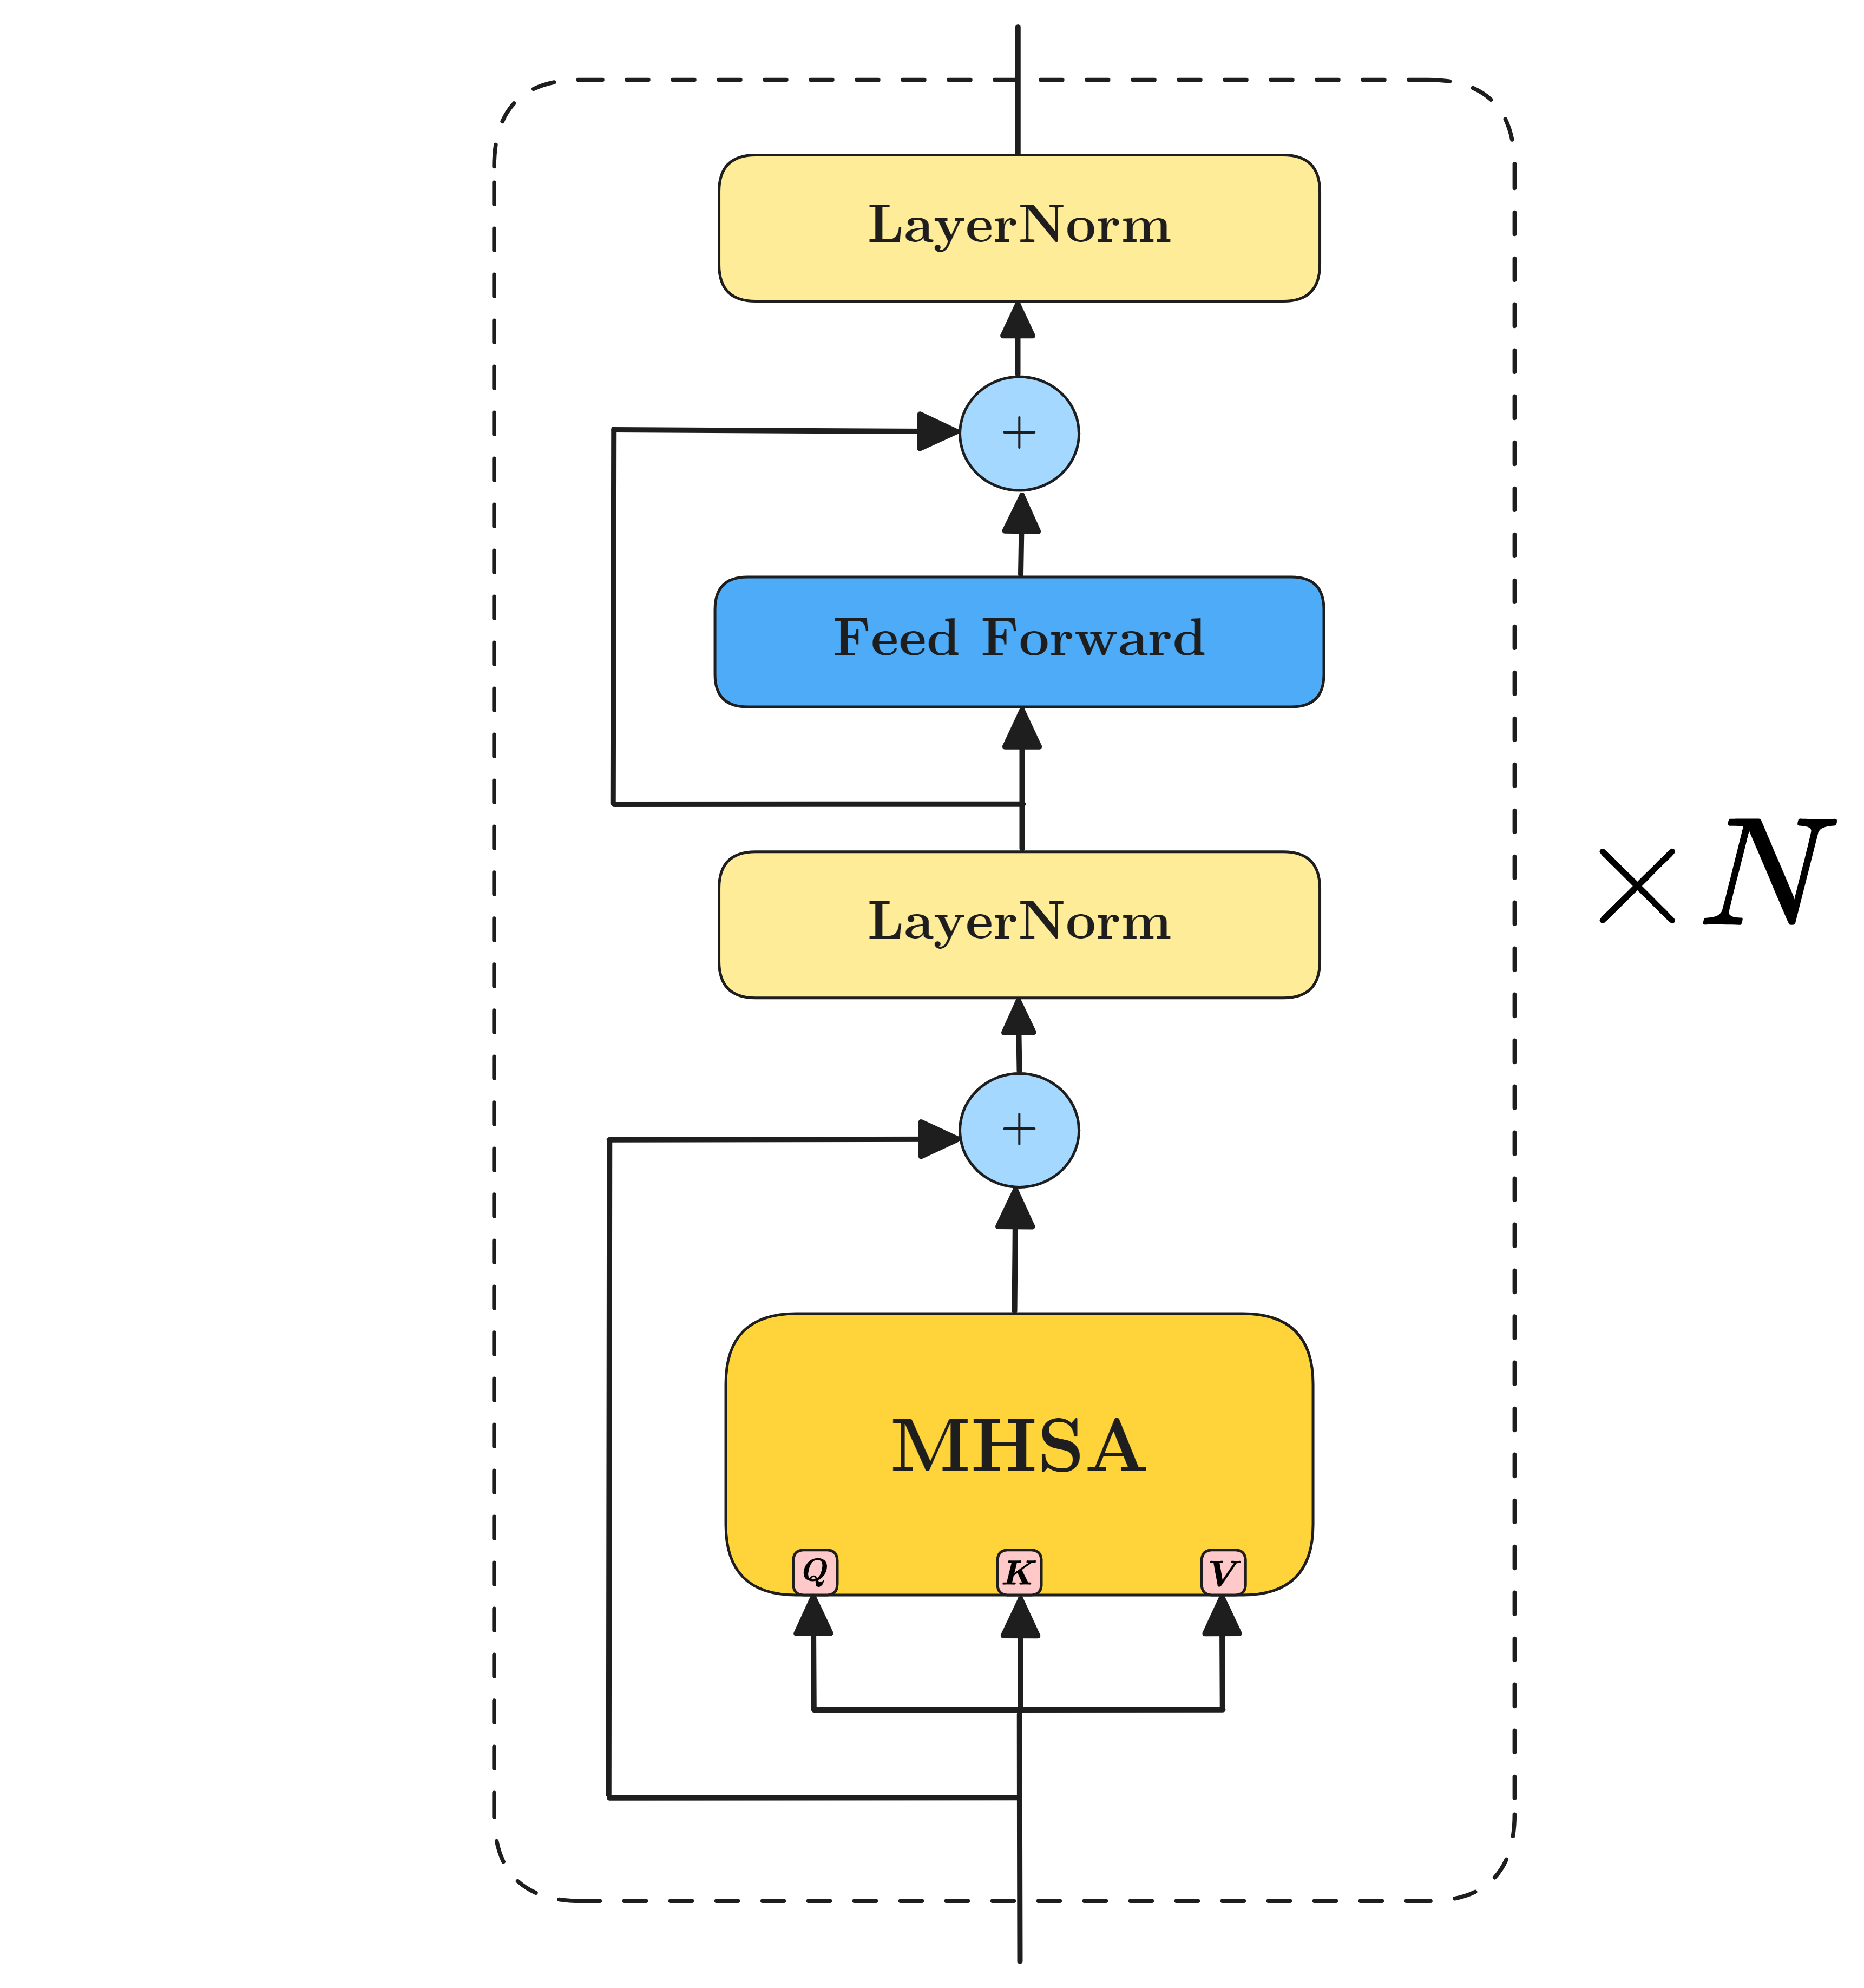
\includegraphics[height=0.5\textwidth]{./encoder.png}
	\caption{Transformer Encoder \parencite{vaswani2017attention}}
	\label{fig:encoder}
\end{figure}

\autoref{fig:encoder} shows the encoder of the transformer model. The encoder is composed of a stack of $N$ identical layers. Each layer is composed of two sub-layers, the MHSA and a simple feed-forward network. The output of each sub-layer is $\text{LayerNorm}(x + \text{Sublayer}(x))$ where $x$ is the input to the sub-layer. To dissect this, we first add the input from the sub-layer to the output of the sub-layer, this is called a \emph{residual} connection. It allows the information from the input to bypass the sublayer and be passed to the next layer, thus preventing the network from losing information about the input. This is then passed through a layer normalization layer. The layer normalization layer normalizes the output (so each row) of the sub-layer to have a mean of 0 and a standard deviation of 1. e.g consider a row of the output of the sub-layer $\bm{h} \elof{1}{D}$, the layer normalization layer will normalize this row as follows:

\begin{align*}
	\bm{h}_{i}\isup{norm} & =  \frac{\bm{h}_i - \mu}{\sigma}\\
	\mu &= \frac{1}{D}\sum_{i=1}^{D} h_i\\
	\sigma &= \sqrt{\frac{1}{D}\sum_{i=1}^{D} (h_i - \mu)^2}
\end{align*}

\noi The final output of the encoder is the output of the last layer which shall be denoted as $\bm{Y} \elof{N}{D}$.

\subsection{Decoder}

\begin{figure}[H]
	\centering
	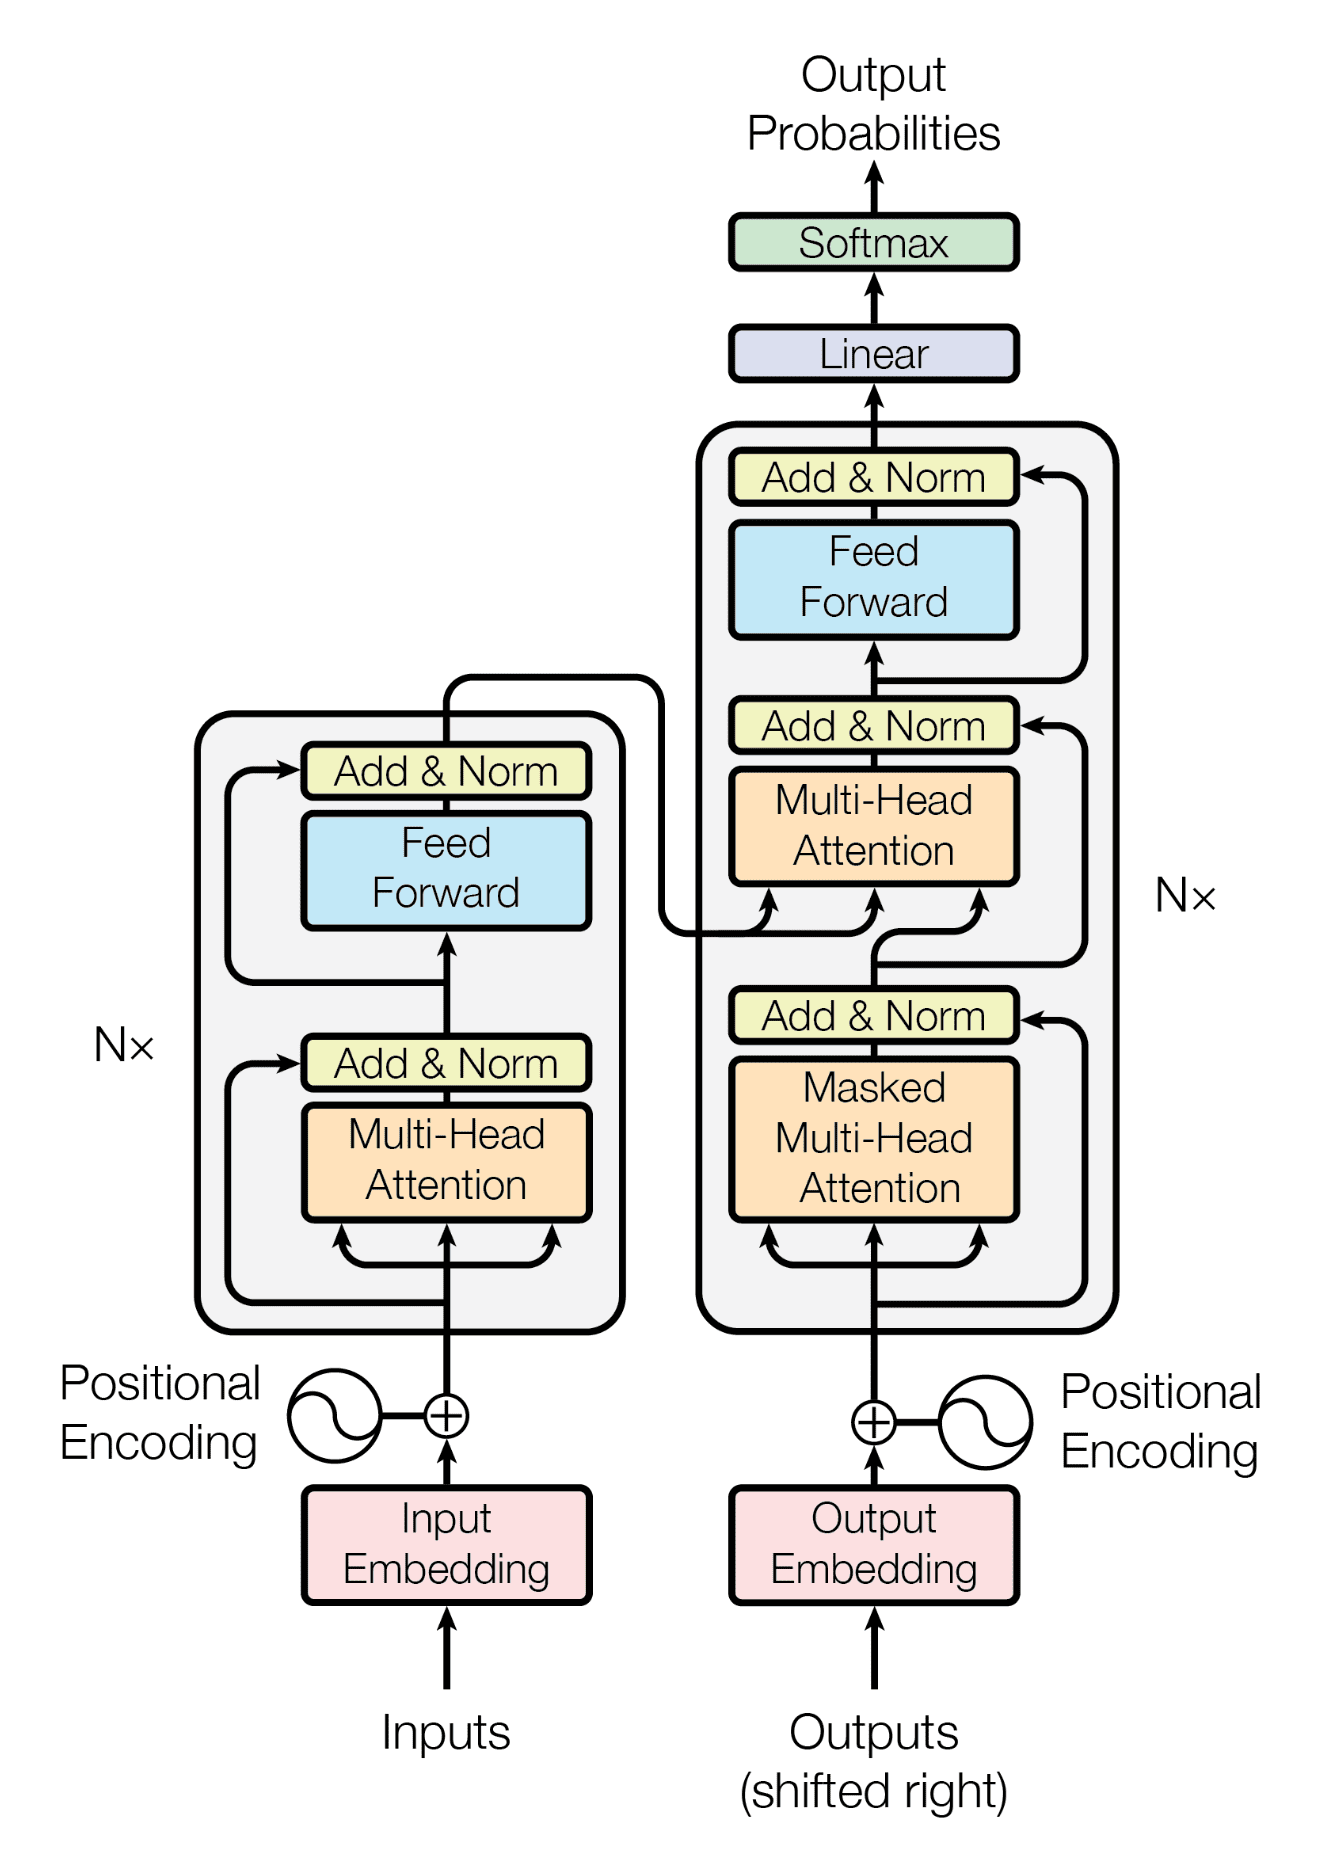
\includegraphics[height=0.6\textwidth]{./transformer.png}
	\caption{Transformer \parencite{vaswani2017attention}}
	\label{fig:transformer}
\end{figure}

The transformer architecture is shown in \autoref{fig:transformer}, the decoder is very similar to the encoder, with a few small differences. We now have an additional block called the \emph{Masked Multi-Head Self-Attention} (M-MHSA). The M-MHSA is identical to the MHSA except that the attention matrix $\bm{A}$ is masked so that the decoder can only attend to previous positions in the sequence. This is done by setting the value of the scaled dot product $\bm{QK^T}/\sqrt{d_k}$ to $-\infty$ for all positions in the sequence that are greater than the current position. Then when the softmax is applied, these values will be $0$ and thus the decoder will not attend to these positions. An example of this is shown below:

\begin{equation}
	\begin{bmatrix}
		0.2 & 0.3 & 0.5 & 0.1 \\
		0.1 & 0.2 & 0.7 & 0.0 \\
		0.3 & 0.4 & 0.2 & 0.1 \\
		0.1 & 0.2 & 0.3 & 0.4 \\
	\end{bmatrix} + 
	\begin{bmatrix}
		0 & -\infty & -\infty & -\infty \\
		0 & 0 & -\infty & -\infty \\
		0 & 0 & 0 & -\infty \\
		0 & 0 & 0 & 0 \\
	\end{bmatrix}
	\xrightarrow{\text{softmax}}
	\begin{bmatrix}
		1 & 0 & 0 & 0 \\
		0.5 & 0.5 & 0 & 0 \\
		0.4759 & 0.3092 & 0.2148 & 0 \\
		0.2824 & 0.3072 & 0.3333 & 0.0771 \\
	\end{bmatrix}
\end{equation}



This ensures that the decoder can only attend to previous positions in the sequence. The M-MHSA is used in the first sub-layer of the decoder. 

The second sub-layer of the decoder is the MHSA, this is identical to the MHSA in the encoder however the keys and values come from the \textbf{encoder output} $\bm{Y}$ and the queries come from the \textbf{output of the M-MHSA sub-layer}. Intutively the encoder learns the attention of the input sequence and the decoder learns how to use query the encoder output to generate the output sequence.
\eq{
	\text{MHSA}_{dec} = \text{MHSA}(\bm{Q_{dec}}, \bm{K_{enc}}, \bm{V_{enc}})
}

The output of the $\text{MHSA}_{dec}$ is then passed through a feed-forward network and layer normalization layer as per usual. This is repeated $N$ times and the output of the final layer is the output of the decoder. This final output is then passed through a linear layer which transforms the decoder output $\elof{N}{D}$ to the output vocabulary size $\elof{N}{\mathcal{V}}$ where $\mathcal{V}$ is the vocabulary of the output language i.e the set of all possible words in the output language. The output of this linear layer is then passed through a softmax layer to generate the final predictive probability distribution over the output vocabulary. We select the word with the highest probability as the predicted word.


\subsection{Training}

The transformer is trained using teacher forcing. Teacher forcing is a technique used in sequence-to-sequence models where the model is trained to predict the next token in the sequence given the previous tokens. This is done by feeding the model the previous tokens and then the next token in the sequence. For example if we want to translate the sentence \texttt{I live in Paris} to French, we would feed the model the tokens \texttt{I} in the encoder and a start token \texttt{<start>} in the decoder and see if it can predict the translated token \texttt{Je}, we then feed correct token \texttt{Je} into the decoder and see if it can predict the next token \texttt{vis} and so on. This forces the model to learn the correct translation of the sentence as we use the correct target tokens to generate a loss function ($\mathcal{L}$) which the transformer decoder optimizes.

The table below shows the training procedure for the translation example. 

\begin{table}[H]
	\centering
	\begin{tabular}{lll}
	\toprule
	{Encoder Input} & {Decoder Input} & {Loss} \\
	\midrule
	\texttt{I}                     & \texttt{<start>} & $\mathcal{L}$(\texttt{pred1}, \texttt{Je}) \\
	\texttt{live}                  & \texttt{Je}                     & $\mathcal{L}$(\texttt{pred2}, \texttt{vis}) \\
	\texttt{in}                    & \texttt{vis}                    & \ldots \\
	\ldots                & \ldots                 & \ldots \\
	\bottomrule
	\end{tabular}
	\end{table}

\subsection{Inference}

After we have trained our model, we can use it for inference. The methodology is similar to the training, however, the decoder output receives the previously predicted token as input instead of the correct target token. This is shown in the table below.

\begin{table}[H]
	\centering
	\begin{tabular}{lll}
	\toprule
	{Encoder Input} & {Decoder Input} & {Decoder Output} \\
	\midrule
	\texttt{I}                     & \texttt{<start>} & \texttt{pred1} \\
	\texttt{live}                  & \texttt{pred1}                     & \texttt{pred2} \\
	\texttt{in}                    & \texttt{pred2}                    & \ldots \\
	\ldots                & \ldots                 & \ldots \\
	\bottomrule
	\end{tabular}
	\end{table}
	


\ifSubfilesClassLoaded{%
    \printbibliography{}
}{} 


\end{document}